%   % !TEX root = ../../VIII,3_Rahmen-TeX_9-0.tex
%  
%   Band VIII, 3 N.~?? 	
%   Signatur/Tex-Datei:	LH_37_05_191-192
%   RK-Nr. 	57269
%   Datierung:		10. (20.) Juni 1677 eigh.
%   edlabels:			4
%   Diagramme: 		3
%
%
%
\selectlanguage{ngerman}
\frenchspacing
%
\begin{ledgroupsized}[r]{120mm}
\footnotesize
\pstart
\noindent\textbf{Überlieferung:}
\pend
\end{ledgroupsized}
%
\begin{ledgroupsized}[r]{114mm}
\footnotesize
\pstart \parindent -6mm
\makebox[6mm][l]{\textit{L}}%
Konzept:
LH~XXXVII~5~Bl.~191\textendash192. 
Ein Bogen~4\textsuperscript{o}; Ränder beschnitten; Papiererhaltungsmaßnahmen.
Vier Seiten.
%Diverses.
\pend
\end{ledgroupsized}
%
\begin{ledgroupsized}[r]{114mm}
\footnotesize
\pstart
\parindent -6mm
\makebox[6mm][l]{\textit{E}}%
\textsc{Fichant} 1994, S.~375\textendash378\cite{01056}.
\pend%
\end{ledgroupsized}
%
%
%
\vspace{5mm}
\begin{ledgroup}
\footnotesize
\pstart
\noindent%
\textbf{Datierungsgründe:}
Sowohl das vorliegende Konzept als auch N.~\ref{RK57270} sind eigh.\ auf den 10.\ (20.) Juni 1677 datiert.
%
Der Großteil von N.~\ref{RK57269} ist der Einführung und Besprechung der Schiffsanalogie als 
%
Hilfsmittel zur Stoßanalyse gewidmet.
%
Leibniz bezieht sich in N.~\ref{RK57270} ausdrücklich auf diese Analogie
%
(siehe bspw.\ S.~\refpassage{37_05_157-158_5a}{37_05_157-158_5b}),
%
die er dort allerdings nicht eigens einführt, sondern lediglich voraussetzt.
%
Dieser Umstand lässt auf die spätere Entstehung von N.~\ref{RK57270} gegenüber N.~\ref{RK57269} schließen.%
\pend
%
%
\pstart
Die Analogie des fahrenden Schiffs, auf dem zwei Körper zusammenstoßen und das vom Ufer aus betrachtet wird, 
%
bietet erstens eine empirische Bestätigung des Relativitätsprinzips, dem beim elastischen Stoß folgende Annahme entspricht:
%
Bei einem beliebigen geraden Stoß zweier gleichförmig bewegter Körper
%
kann die gemeinsame (gleichförmige) Bewegung des Systems, d.h.\ die des gemeinsamen Schwerpunkts, 
%
von denen der einzelnen Körper abgezogen werden,
%
ohne die Wirkungen des Stoßes zu verändern.
%
Zweitens verdeutlicht die Analogie die auf dem Relativitätsprinzip fußende Methode der Stoßanalyse:
%
Nach Abzug der gleichförmigen Bewegung des Schwerpunkts
%
(bzw., in der Analogie, der des Schiffs)
%
erhält man immer einen einfachen Stoßfall, in dem die Geschwindigkeiten der Körper sich reziprok zu den Massen verhalten, 
%
und dessen Ausgang der Austausch ihrer Impulse ist.
%
%Daraus folgt auch die Erhaltung der relativen Geschwindigeit der Körper.
%
Die resultierende Bewegung kann anschließend wieder mit der des Schwerpunkts (bzw.\ Schiffes) zusammengesetzt werden,
%
um die Geschwindigkeiten der Körper nach dem Stoß zu erhalten
%
(in der Analogie: Man beobachtet den Stoß auf dem Schiff vom Ufer aus).
%
%
\pend
%
\pstart
%
Das vorliegende Konzept ist eins der frühesten bekannten Texten, in denen Leibniz die Schiffsanalogie einführt, 
%
sie ausführlich anwendet, 
%
und sich mit ihrer theoretischen Grundlage 
%
(dem Relativitätsprinzip bzw.\ der Zusammensetzung von Bewegungen) kritisch auseinandersetzt.
%
(\protect\vphantom)Ähnliche Ausführungen bietet das Stück \textit{LSB} VI,~3 N.~6, 
das wahrscheinlich zwischen 1673 und 1676, vielleicht aber erst in der Hannoveraner Zeit entstand; 
siehe auch die auf den Zeitraum 1677 bis Winter 1680/81 datierbaren Konzepte 
\textit{LSB} VI,~4 N.~359 und N.~362.\protect\vphantom()
%
Der Ansatz ist nicht originell,
%
sondern war Leibniz mit Sicherheit bereits aus den Publikationen von \protect\index{Namensregister}{\textso{Wallis} (Wallisius), John 1616\textendash1703}Wallis und \protect\index{Namensregister}{\textso{Mariotte}, Edme, Seigneur de Chazeuil ca. 1620\textendash1684}Mariotte
%
bekannt, die er in Paris gelesen und exzerpiert hatte
(siehe \cite{01292}\textit{LSB} VIII, 2 N.~50 und  \cite{01343}\textit{LSB} VIII, 2 N.~8, bes.\ S.~82\textendash93).
%
Beide Autoren waren nach dieser Methode verfahren und hatten ihre Annahmen mithilfe der Schiffsanalogie veranschaulicht:
%
siehe \protect\index{Namensregister}{\textso{Wallis} (Wallisius), John 1616\textendash1703}\textsc{J.~Wallis}, 
\cite{00301}\textit{Mechanica}, London 1670\textendash1671, Pars~III, Cap.~XI, Prop.~VIII und Scholium, S.~669f. (\cite{01008}\textit{WO} I, S.~1007f.) und
%
\protect\index{Namensregister}{\textso{Mariotte}, Edme, Seigneur de Chazeuil ca. 1620\textendash1684}%
\textsc{E.~Mariotte}, %
\cite{00311}\title{Traité de la percussion}, Première Partie, Prop.~III (Second principe d'experience), S.~25\textendash29.
%
%
%
%
\pend
%
\pstart
Mindestens ebenso wichtig waren das Relativitätsprinzip und die Schiffsanalogie für Huygens' Herleitung der Stoßgesetze gewesen; 
%
sie liegen der Abhandlung \cite{00530}\glqq De motu corporum ex percussione\grqq\ (\textit{HO} XVI, S.~29\textendash91)
%
und dem Aufsatz 
%
\cite{02037}\glqq De motu corporum ex mutuo impulsu hypothesis\grqq\ (\cite{00113}\textit{HO} VI, Nr.~1693, S.~336\textendash343)
%
zugrunde, die spätestens um 1669 abgeschlossen (siehe \textit{HO} XVI, S.~10\textendash14),
%
aber zum Zeitpunkt der Abfassung des vorliegenden Konzepts
%
unveröffentlicht waren.
%
\cite{00530}\glqq De motu\grqq\ erschien erst 1703
%
(\protect\vphantom)in den \cite{02076}\textit{Opuscula postuma}, 
%
hrsg.\ von \protect\index{Namensregister}{\textso{Volder} (Volter, Wolder), Burchard (Burcher) de 1643\textendash1709}B.\ De~Volder 
%
und \protect\index{Namensregister}{\textso{Fullenius}, Bernardus 1640\textendash1707}B.~Fullenius, Leiden 1703, 
%
S.~367\textendash398\protect\vphantom(),
%
während die \glqq Hypothesis\grqq\  weiterhin ungedruckt blieb.
%
Zwar hatte Huygens letzteren Aufsatz für die Publikation vorgesehen und
%
am 5.\ Januar 1669 bei der \textit{Royal Society} in Beantwortung der Frage nach den Stoßgesetzen eingereicht,
%
doch erhielt \protect\index{Namensregister}{\textso{Oldenburg} (Grubendol), Heinrich 1618\textendash1677}H.~Oldenburg den Text
%
nicht rechtzeitig und konnte ihn nicht neben den Antworten von \protect\index{Namensregister}{\textso{Wallis} (Wallisius), John 1616\textendash1703}\cite{01065}Wallis und \protect\index{Namensregister}{\textso{Wren} (Wrennus), Christopher 1632\textendash1723}\cite{01066}Wren
%
(\cite{00158}\textit{PT} III, Januar 1669, S.~864\textendash866 und S.~867f.)
%
drucken (siehe \textit{HO} XVI, S.~171\textendash178 und \textit{HO} VI, S.~334f.).
%
Daraufhin publizierte Huygens zwei stark gekürzte Fassungen der \glqq Hypothesis\grqq\
%
(\protect\vphantom)\cite{00529}\glqq Regles du mouvement dans la rencontre des corps\grqq, \cite{00157}\textit{JS}, Pariser Ausgabe, 18.~März 1669, S.~22\textendash24 und \glqq A summary account of the laws of motion\grqq, \cite{00158}\textit{PT} IV, April 1669, S.~925\textendash928\protect\vphantom(),
%
in denen er sich auf eine knappe Darstellung der Ergebnisse beschränkte, 
%
ohne Hinweise auf ihre Herleitung aus dem Relativitätsprinzip zu geben.
%
Leibniz hat beide Artikel exzerpiert
%
(siehe N.~\ref{RK57267-2} von März\textendash Mai 1677 bzw.\ \cite{02025}\textit{LSB} VI, 2 N.~38\textsubscript{1}).
%
Er assoziiert bereits um 1677 die äquivalenten Stoßregeln von \protect\index{Namensregister}{\textso{Wallis} (Wallisius), John 1616\textendash1703}Wallis, \protect\index{Namensregister}{\textso{Mariotte}, Edme, Seigneur de Chazeuil ca. 1620\textendash1684}Mariotte und \protect\index{Namensregister}{\textso{Huygens} (Hugenius, Ugenius, Hugens, Huguens), Christiaan 1629\textendash1695}Huygens
%
primär mit letzterem Autor und nennt sie zuweilen schlicht \glqq regulae Hugenianae\grqq\
%
(bspw.\ auf S.~\refpassage{37_05_191-192_4a}{37_05_191-192_4b} oder in N.~\ref{RK57274} und N.~\ref{RK57276}).
%
Noch Jahre später spricht er \protect\index{Namensregister}{\textso{Huygens} (Hugenius, Ugenius, Hugens, Huguens), Christiaan 1629\textendash1695}Huygens die Urheberschaft der Stoßgesetze
%
wie auch der Schiffsanalogie zu: Der
%
Brief an \protect\index{Namensregister}{\textso{Le Bovier de Fontenelle}, Bernard 1657\textendash1757}Fontenelle vom 6.\ Januar 1703
%
enthält eine Bemerkung über die anerkannte Stoßregel, \glqq que dernierement un homme ingenieux chez vous 
%
\lbrack d.h.\ \protect\index{Namensregister}{\textso{Parent}, Antoine 1666\textendash1716}Antoine Parent\rbrack\ 
%
a expliquée comme M.~Hugens par la methode du bateau\grqq\ (LBr~68 Bl.~139\textendash140; erscheint in \textit{LSB} II, 4).
%
Zu diesem Zeitpunkt war die posthume Ausgabe von \glqq De motu\grqq\ noch nicht erschienen; 
%
ein von \protect\index{Namensregister}{\textso{Volder} (Volter, Wolder), Burchard (Burcher) de 1643\textendash1709}De~Volder für Leibniz bestimmtes Exemplar 
%
(\textit{GWLB}, Nm-A~403, mit Leibnizens Marginalien) erreichte ihn erst im Sommer über 
%
\protect\index{Namensregister}{\textso{Mencke} (Menken, Menkenius, Menque), Otto 1644\textendash1707}O.~Mencke 
%
(\protect\vphantom)siehe den Brief an Johann Bernoulli vom 3.\ Juli 1703: Basel \textit{Universitätsbibl}.\ L~Ia 19 Bl.~205\textendash206; der Brief erscheint in \textit{LSB} III, 9\protect\vphantom().
%
%%
\pend
%
\pstart
Über die Möglichkeit von Leibniz' Kenntnis der Huygens'schen Thesen zur Zeit der Abfassung 
%
von N.~\ref{RK57269} kann folgendes festgestellt werden.
%
Es gibt keine Belege für eine Leibniz'sche Lektüre der beiden unveröffentlichten Werke bis 1677;
%
der rege persönliche Austausch zwischen \protect\index{Namensregister}{\textso{Huygens} (Hugenius, Ugenius, Hugens, Huguens), Christiaan 1629\textendash1695}Huygens und ihm in Paris\protect\index{Ortsregister}{Paris} ist bekannt;
%
aus dem Zeitraum Juli 1676 bis Mitte September 1679 sind keine Briefe erhalten.
%
Auch unabhängig von der Lektüre der Manuskripte könnte Leibniz auf einem zusätzlichem Wege
%
von \protect\index{Namensregister}{\textso{Huygens} (Hugenius, Ugenius, Hugens, Huguens), Christiaan 1629\textendash1695}Huygens' Thesen erfahren haben: Diese dürften nach seinen Vorträgen über die Stoßlehre 
%
von Januar 1668 in der Académie des Sciences  (siehe \textit{HO} XVI, S.~182\textendash186)
%
in Pariser Gelehrtenkreisen bekannt gewesen sein.
%
Tatsächlich unterstellte \protect\index{Namensregister}{\textso{Huygens} (Hugenius, Ugenius, Hugens, Huguens), Christiaan 1629\textendash1695}Huygens \protect\index{Namensregister}{\textso{Mariotte}, Edme, Seigneur de Chazeuil ca. 1620\textendash1684}Mariotte, 
%
sich die wichtigsten Ideen und Ergebnisse, \glqq quae in consessu Eruditorum in Bibliotheca Regia adductis demonstrationibus comprobaveram\grqq,
%
angeeignet und den \textit{Traité} von 1673 ganz auf ihrer Grundlage gebaut zu haben.
%
Noch um 1704 wird Leibniz mit ähnlichen Argumenten seinen Vorwurf eines Huygens-Plagiats gegen 
%
\protect\index{Namensregister}{\textso{Parent}, Antoine 1666\textendash1716}A.~Parents \cite{01500}\textit{Élémens} von 1700
%
begründen (\protect\vphantom)siehe die editorische Vorbemerkung zu N.~\ref{Parent_intro}\protect\vphantom().
%
Es kann davon ausgegangen werden, dass Leibniz von \protect\index{Namensregister}{\textso{Huygens} (Hugenius, Ugenius, Hugens, Huguens), Christiaan 1629\textendash1695}Huygens' Académie-Vorträgen und von der Verbreitung seiner Thesen wusste;
%
möglicherweise war er auch über die Inhalte informiert.
%
Abschließend kann festgehalten werden, dass eine Kenntnis der \protect\index{Namensregister}{\textso{Huygens} (Hugenius, Ugenius, Hugens, Huguens), Christiaan 1629\textendash1695}Huygens'schen Hypothesen und seiner (Schiffs-)Methode
%
als Quelle von N.~\ref{RK57269} nicht angenommen werden muss, 
%
sie aber aus den genannten Gründen nicht auszuschließen ist.
%
\pend
%
\end{ledgroup}
%
\newpage
%
%
\selectlanguage{latin}
\frenchspacing
% \newpage%
\vspace{8mm}
\count\Bfootins=1100%
\count\Afootins=1100%
\count\Cfootins=1100
\pstart%
\normalsize%
\noindent%
\lbrack191~r\textsuperscript{o}\rbrack\
\pend 
%
\pstart
\raggedleft
10 Junius 1677
\pend
%
%
\vspace{1.0em} %%%%%%%%% Diagramm 1
\centerline{%
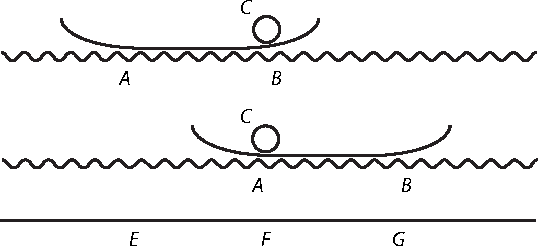
\includegraphics[width=0.7\textwidth]{%
gesamttex/edit_VIII,3/images/LH_37_05_191-192_d1_191r.pdf%
}} 
\vspace{0.5em}
\centerline{%
\lbrack\textit{Fig.~1}\rbrack%
}
% \newpage%
\vspace{1.5em}
%
\pstart \noindent
Tutum non est uti motuum compositionibus,%
\protect\index{Sachverzeichnis}{compositio motuum} quod hoc
exemplo ostendam. Sit %
navicula\protect\index{Sachverzeichnis}{navicula} \textit{AB} in aqua labens
secundo flumine,%
\protect\index{Sachverzeichnis}{flumen} ita ut si e %
ripa\protect\index{Sachverzeichnis}{ripa} immota \textit{EFG} spectetur
transferatur \textit{AB} ex \textit{EF} in \textit{FG}. Sit in %
navicula\protect\index{Sachverzeichnis}{navicula} corpus \textit{C}, quod
eadem celeritate moveatur a prora %
navis\protect\index{Sachverzeichnis}{navis} \textit{B}, ad puppim, directe, qua
%
navis\protect\index{Sachverzeichnis}{navis} in flumine%
\protect\index{Sachverzeichnis}{flumen} procedit, patet ergo cum %
navis\protect\index{Sachverzeichnis}{navis} ex 
%%
\textit{EF} venit
in \textit{FG}, 
%
\edtext{corpus \textit{C}}{\lemma{corpus}\Bfootnote{\textit{(1)}~\textit{B} \textit{(2)}~\textit{C}~\textit{L}}} 
%
ex \textit{B} venisse in \textit{A}. Jam antea \textit{B} respondebat
puncto immobili \textit{F} in ripa, nunc \textit{A}, respondet eidem, ergo
%
\edtext{corpus \textit{C} adhuc}{\lemma{corpus \textit{C}}\Bfootnote{\textit{(1)}~semper \textit{(2)}~adhuc~\textit{L}}} 
%
ipsi \textit{F} respondet, ac proinde ex %
ripa\protect\index{Sachverzeichnis}{ripa} spectanti
motu carere videbitur. Quaeritur jam an absolute 
loquendo %
motus\protect\index{Sachverzeichnis}{motus} aliquis corpori \textit{C} tribuendus 
%
\edtext{sit: et}{\lemma{sit:}\Bfootnote{\textit{(1)}~videtur enim reapse \textit{(2)}~et~\textit{L}}}
%
videri potest reapse quiescere, cum eadem
%
celeritate regrediatur,
%
qua progreditur. 
%
\edtext{Verum absolutum}{\lemma{Verum}\Bfootnote{\textit{(1)}~quia \textit{(2)}~absolutum~\textit{L}}}
%
illud in motu,%
\protect\index{Sachverzeichnis}{absolutum in motu} quod vim,%
\protect\index{Sachverzeichnis}{vis} sive potentiam%
\protect\index{Sachverzeichnis}{potentia} voco, spectanti
omnino dicendum est moveri, et quidem duplici contrarioque motu,%
\protect\index{Sachverzeichnis}{motus duplex et contrarius}
ac proinde tantum abest ut quiescat, ut contra potius duplicatam
habeat potentiam,%
\protect\index{Sachverzeichnis}{potentia} quod sic ostendo: ponatur ipsi in navi%
\protect\index{Sachverzeichnis}{navis} moto occurrere
aliquod elaterium in navi fixum,%
\protect\index{Sachverzeichnis}{elaterium in navi fixum} et
%
\edtext{hoc elaterium\protect\index{Sachverzeichnis}{elaterium}}{\lemma{hoc}\Bfootnote{\textit{(1)}~ab \textit{(2)}~elaterium~\textit{L}}}
%
ab eo tendi
atque ita potentiam%
\protect\index{Sachverzeichnis}{potentia} ipsius insumi, hoc facto in navi%
\protect\index{Sachverzeichnis}{navis} quiescet, 
%
\edtext{et nihilominus}{\lemma{et}\Bfootnote{\textit{(1)}~ponamus porro \textit{(2)}~nihilominus~\textit{L}}} 
%
motum cum navi exercebit, quasi pars ejus, ac potentiam%
\protect\index{Sachverzeichnis}{potentia}
%
navis\protect\index{Sachverzeichnis}{navis} augebit, quoniam ejus pondus%
\protect\index{Sachverzeichnis}{pondus} sive molem solidam%
\protect\index{Sachverzeichnis}{molis solida} auget. Itaque
si %
navis\protect\index{Sachverzeichnis}{navis} inter procedendum in aliud 
%
\edtext{corpus quiescens\protect\index{Sachverzeichnis}{corpus quiescens} aequalis}{\lemma{}\Bfootnote{quiescens \textit{erg.}~\textit{L}}} 
%
\edtext{ponderis ripae connexum%
\protect\index{Sachverzeichnis}{corpus ripae connexum} impingat}{\lemma{}\Bfootnote{ripae connexum \textit{erg.}~\textit{L}}},
%
eique suam vim%
\protect\index{Sachverzeichnis}{vis}
%
\edtext{tribuat, navis}{\lemma{tribuat,}\Bfootnote{\textit{(1)}~patet \textit{(2)}~navis~\textit{L}}}
%
cum corpore \textit{C} in eo quiescet, 
et %
potentia\protect\index{Sachverzeichnis}{potentia} ipsius \textit{C}, quae partem faciebat %
potentiae\protect\index{Sachverzeichnis}{potentia} navis, erit conservata
%
\edtext{atque in ripam translata}{\lemma{}\Bfootnote{in ripam \textit{erg.}~\textit{L}}}. 
%
Porro si Elaterium%
\protect\index{Sachverzeichnis}{elaterium}
%
\edtext{tensum liberetur adhuc}{\lemma{}\Bfootnote{liberetur \textit{erg.}~\textit{L}}} 
%
potentiam%
\protect\index{Sachverzeichnis}{potentia} suam
etiam in corpus in ripa%
\protect\index{Sachverzeichnis}{ripa} positum, quiescente jam navi, ut supponimus, exercebit,
atque ita manifestum est utramque potentiam%
\protect\index{Sachverzeichnis}{potentia} jam in ripam%
\protect\index{Sachverzeichnis}{ripa}
%%%%%%%%%%%%%%%%%%
%%
\lbrack191~v\textsuperscript{o}\rbrack\
%%
%%%%%%%%%%%%%%%%%%%
immobilem esse translatam; ac proinde absolute loquendo
dicendum esse corpus 
%
\edtext{\textit{C}}{%
\lemma{}%
\Bfootnote{%
\textit{C} %
\textit{erg.~L}%
}}
%
in navi%
\protect\index{Sachverzeichnis}{navis} moveri, etsi is motus e ripa%
\protect\index{Sachverzeichnis}{ripa} 
spectanti non appareat. 
%
\edtext{Itaque spectanda}{\lemma{Itaque}\Bfootnote{\textit{(1)}~motu \textit{(a)}~non \textit{(b)}~aestimanda \textit{(2)}~spectanda~\textit{L}}} 
%
sunt corpora 
proxime 
%
\edtext{ambientia sive}{\lemma{ambientia}\Bfootnote{\textit{(1)}~, ut de navi \textit{(2)}~sive~\textit{L}}}
%
contingentia,%
\protect\index{Sachverzeichnis}{corpora proxime ambientia sive contingentia} ut de alicujus 
corporis motu%
\protect\index{Sachverzeichnis}{motus} et quiete%
\protect\index{Sachverzeichnis}{quies} judicetur.  
%
\edtext{Quemadmodum \protect\index{Namensregister}{\textso{Aristoteles} 384\textendash322 v. Chr.}Aristoteles
%
\edtext{recte advertit}{\lemma{recte}\Bfootnote{\textit{(1)}~dixit \textit{(2)}~ab \textit{(3)}~advertit~\textit{L}}},
%
cum locum\protect\index{Sachverzeichnis}{locus} vocavit %
superficiem ambientis.\protect\index{Sachverzeichnis}{superficies ambientis}}{\lemma{Quemadmodum \lbrack...\rbrack\ ambientis}\Cfootnote{\protect\index{Namensregister}{\textso{Aristoteles} 384\textendash322 v. Chr.}\textsc{Aristoteles}, \cite{00235}\textit{Physica} IV, 4,~212a2\textendash6.}} 
%
Unum enim corpus 
%
\edtext{unicum proprium habet}{\lemma{}\Bfootnote{proprium \textit{erg.}~\textit{L}}}
%
\edtext{locum%
\protect\index{Sachverzeichnis}{locus proprius} una vice, superficiem}{\lemma{}\Bfootnote{una vice \textit{erg.}~\textit{L}}}
%
ambientis;%
\protect\index{Sachverzeichnis}{superficies ambientis} et per consequens
unicum motum proprium,%
\protect\index{Sachverzeichnis}{motus proprius} scilicet separationem ab illa superficie.%
\protect\index{Sachverzeichnis}{superficies ambientis}
\pend 
%
\vspace{2.5em} %%%%%%%%% Diagramm 2
\centerline{%
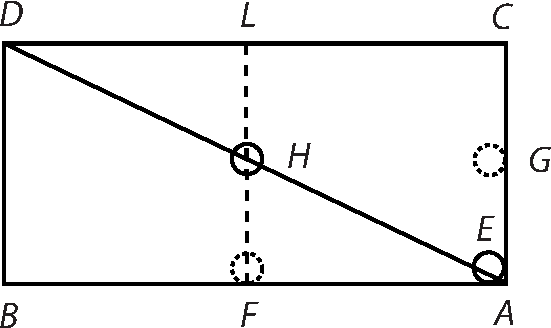
\includegraphics[width=0.45\textwidth]{%
gesamttex/edit_VIII,3/images/LH_37_05_191-192_d2_191v.pdf%
}} 
\vspace{0.5em}
\centerline{%
\lbrack\textit{Fig.~2}\rbrack%
}
\newpage%
\count\Bfootins=1000%
\count\Afootins=1000%
\count\Cfootins=1000
%
%\vspace{1.5em}
%
\pstart
%
\hspace{1mm}\hspace{-1mm}% Trick, weil \edlabel nicht zu \par-Beginn sein darf
\edlabel{37_05_191-192_3a}%
\edtext{Hanc observationem}{\lemma{Hanc}\Bfootnote{\textit{(1)}~regulam non \textit{(2)}~observationem~\textit{L}}}
%
neglexere 
%
\edtext{Clarissimi Viri, qui per motuum compositiones,\protect\index{Sachverzeichnis}{compositio motuum} %
phenomena concursuum\protect\index{Sachverzeichnis}{phaenomena concursuum}%
\protect\index{Sachverzeichnis}{concursus}
explicare conati sunt.}{%
\lemma{Clarissimi \lbrack...\rbrack\ sunt}%	
\Cfootnote{%
%
\protect\index{Namensregister}{\textso{Wallis} (Wallisius), John 1616\textendash1703}\textsc{J.~Wallis}, \cite{00301}\textit{Mechanica}, London 1670\textendash1671, Pars~III, Cap.~XI, S.~660\textendash682 (\cite{01008}\textit{WO} I, S.~1002\textendash1015) und Cap.~XIII, S.~686\textendash707 (\cite{01008}\textit{WO} I, S.~1018\textendash1031);
%
\protect\index{Namensregister}{\textso{Mariotte}, Edme, Seigneur de Chazeuil ca. 1620\textendash1684}%
\textsc{E.~Mariotte}, %
\cite{00311}\title{Traité de la percussion}, \textit{passim}; siehe auch Leibnizens kommentierte Auszüge von März\textendash Mai 1677 (N.~\ref{57267_3}).
%
Möglicherweise spielt Leibniz auch auf \protect\index{Namensregister}{\textso{Huygens} (Hugenius, Ugenius, Hugens, Huguens), Christiaan 1629\textendash1695}Huygens an, der in unveröffentlichten
Texten wie
\cite{00530}\glqq De motu corporum ex percussione\grqq\
(um 1703 posthum erschienen; auch \cite{00113}\textit{HO} XVI, S.~29\textendash91)
und \cite{02037}\glqq De motu corporum hypothesis\grqq\ (\cite{00113}\textit{HO} VI, Nr.~1693, S.~336\textendash343) die Stoßgesetze anhand zusammengesetzter Bewegungen hergeleitet hatte.
Siehe dazu die editorische Vorbemerkung.}}
%
\edtext{Nimirum ipsis nihil refert, utrum dicamus
corpus 
\edtext{\textit{E} ferri celeritate}{%
\lemma{\textit{E} ferri}%
\Bfootnote{%
\textit{(1)}~ex %
\textit{(2)}~celeritate%
~\textit{L}}}
%
et directione \textit{AD}, an
vero 
\edtext{dicamus ferri duobus}{\lemma{dicamus ferri}\Bfootnote{\textit{(1)}~cele \textit{(2)}~celeritate \textit{(3)}~duobus~\textit{L}}}
motibus%
\protect\index{Sachverzeichnis}{motus}
nimirum celeritate et directione \textit{AC}, ac simul 
celeritate et directione \textit{AB}.\edlabel{37_05_191-192_3b}}{%
\lemma{Nimirum \lbrack...\rbrack\  \textit{AB}}%
\Cfootnote{%
Siehe z.B.\
%
\protect\index{Namensregister}{\textso{Huygens} (Hugenius, Ugenius, Hugens, Huguens), Christiaan 1629\textendash1695}\textsc{Huygens},
\cite{02037}\glqq De motu corporum hypothesis\grqq, §3, S.~336;
%
\protect\index{Namensregister}{\textso{Wallis} (Wallisius), John 1616\textendash1703}\textsc{Wallis},
\cite{00301}\textit{Mechanica}, Pars~III, Cap.~XI, Prop.~VIII und Scholium, S.~669f.;
%
\protect\index{Namensregister}{\textso{Mariotte}, Edme, Seigneur de Chazeuil ca. 1620\textendash1684}%
\textsc{Mariotte},
\cite{00311}\textit{Traité de la percussion}, Première Partie, Prop.~III (Second principe d'experience), S.~25\textendash29.
%
Alle drei Autoren veranschaulichen ihre Methoden mithilfe der Schiffsanalogie.}}
%
Cum tamen plurimum intersit,
et posteriore casu multo major sit futura potentia%
\protect\index{Sachverzeichnis}{potentia} corporis
\textit{E}, quam 
%
\edtext{priore. Nam}{\lemma{priore.}\Bfootnote{\textit{(1)}~Ponamus enim \textit{(2)}~Nam~\textit{L}}} 
%
priore casu
super tabula immobili%
\protect\index{Sachverzeichnis}{tabula immobilis} \textit{ABDC} fertur corpus 
%
\edtext{\textit{A}, directione ac potentia}{\lemma{\textit{A},}\Bfootnote{\textit{(1)}~recta ac \textit{(2)}~directione \textit{(a)}~\textit{A} \textit{(b)}~ac potentia~\textit{L}}}
%
ut \textit{AD}, posteriore modo intelligetur super immobili tabula%
\protect\index{Sachverzeichnis}{tabula immobilis} \textit{ABDC} procedere
regula
%
\edtext{\textit{CA} per \textit{LF} in \textit{DB}, directione}{\lemma{\textit{CA}}\Bfootnote{\textit{(1)}~in \textit{(2)}~per \textit{LF} \textbar\ in \textit{DB} \textit{erg.}\ \textbar\ , directione~\textit{L}}}
% 
%
\edtext{ac celeritate \textit{AB} et secum ferre corpus}{\lemma{}\Bfootnote{et secum ferre corpus \textit{erg.}~\textit{L}}}, 
%
atque interim
super ipsa regula procedere corpus
%
\edtext{ex \textit{A} per \textit{G} versus \textit{C}, directione}{\lemma{\textit{A}}\Bfootnote{\textit{(1)}~in \textit{G} \textit{(2)}~per \textit{G} versus \textit{C}, \textit{(a)}~celeritate et \textit{(b)}~directione~\textit{L}}}
%
ac celeritate 
%
\edtext{\textit{AC}. Ajo potentiam corporis \textit{E} priori modo sumti,}{\lemma{\textit{AC}.}\Bfootnote{\textit{(1)}~Ergo prio \textit{(2)}~Ajo \textit{(a)}~priore modo \textit{(b)}~potentiam corporis \textit{(aa)}~quae priore modo sumta \textit{(bb)}~priore modo sumtam \textit{(cc)}~\textit{E} priore modo sumti,~\textit{L}}}
%
 ad eam quae posteriore modo
deprehenditur esse ut \textit{AD} ad $BA + AC$, unde facile 
motum perpetuum%
\protect\index{Sachverzeichnis}{motus perpetuus} exhibere possem, si nihil referret
%
\edtext{\lbrack utrum\rbrack}{%
\lemma{}%
\Bfootnote{%
utrum %
\textit{erg.~Hrsg.}%
}}
%
posteriore
modo an priore uteremur. %
\pend
%
\pstart
Possunt tamen inservire hae motuum compositiones%
\protect\index{Sachverzeichnis}{compositio motuum} ad explicandas directiones,%
\protect\index{Sachverzeichnis}{directio} modo id fiat salva potentiae
summa.%
\protect\index{Sachverzeichnis}{summa potentiae} %
\pend
%
\pstart
Itaque in materia concursuum%
\protect\index{Sachverzeichnis}{concursus} si duo 
%
\edtext{corpora \lbrack192~r\textsuperscript{o}\rbrack\ inaequali}{\lemma{corpora}\Bfootnote{\textit{(1)}~eadem  \lbrack192~r\textsuperscript{o}\rbrack\ \textit{(2)}~inaequali~\textit{L}}}
%
celeritate ferentur in eandem plagam, ita ut quod
praecedit sit tardius, quo scilicet quod sequitur possit 
ipsum assequi, tunc intelligi potest, id quod antecedit quiescere in navi,%
\protect\index{Sachverzeichnis}{navis} in qua id
quod sequitur, in ipsum incurrit excessu celeritatis,%
\protect\index{Sachverzeichnis}{excessus celeritatis} %
navis\protect\index{Sachverzeichnis}{navis} autem
feretur celeritate tardioris.%
\pend
\newpage
%
%
%\vspace{2.0em} %%%%%%%%% Diagramm 3
\centerline{%
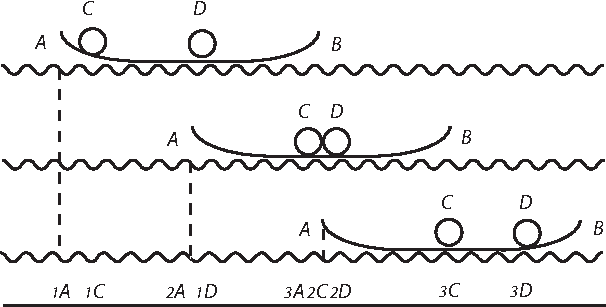
\includegraphics[width=0.8\textwidth]{%
gesamttex/edit_VIII,3/images/LH_37_05_191-192_d3_192r.pdf%
}} 
\vspace{0.5em}
\centerline{%
\lbrack\textit{Fig.~3}\rbrack%
}
% \newpage%
\vspace{1.5em}
%
\pstart
Sit
%
\edtext{celeritas tardioris}{\lemma{celeritas}\Bfootnote{\textit{(1)}~navis \textit{(2)}~tardioris~\textit{L}}}
%
$ {\scriptstyle 1}D{\scriptstyle 2}D$\lbrack,\rbrack\
detur eadem
%
\edtext{navi, seu \textit{{\scriptsize1}A{\scriptsize2}A}}{\lemma{}\Bfootnote{seu \textit{erg.}~\textit{L}}}
%
aequalis sit \textit{{\scriptsize1}D{\scriptsize2}D}, quiescet corpus \textit{D} in navi, 
corpus \textit{C} vero 
%
\edtext{feretur celeritate \textit{{\scriptsize1}C{\scriptsize2}C}}{\lemma{feretur}\Bfootnote{\textit{(1)}~celeritatum summa \textit{(2)}~celeritate \textit{{\scriptsize1}C{\scriptsize2}C}~\textit{L}}},
%
quae est
%%
$\underset{\phantom{{\scriptstyle 1}C}\, \displaystyle\text{vel}\ + {\scriptstyle 1}D{\scriptstyle 2}D}{{\scriptstyle 1}C{\scriptstyle 1}D + {\scriptstyle 1}A{\scriptstyle 2}A}$.
%%
\rule[0cm]{0mm}{10pt}Post concursum perget corpus \textit{D}
%
\edtext{celeritate quam}{\lemma{celeritate}\Bfootnote{\textit{(1)}~in n \textit{(2)}~quam~\textit{L}}}
%
quiescens in navi%
\protect\index{Sachverzeichnis}{navis}
%
\edtext{accepit, nempe}{\lemma{accepit,}\Bfootnote{\textit{(1)}~et corpus \textit{C} celeritate qu \textit{(2)}~nempe~\textit{L}}}
%
\textit{DB} et praeterea celeritate
navis \textit{{\scriptsize2}A{\scriptsize3}A}, seu
%%
${\scriptstyle 2}D{\scriptstyle 3}D \ \sqcap \ {\scriptstyle 2}A{\scriptstyle 3}A + DB$\lbrack,\rbrack\
%%
corpus \textit{C} vero residua,
et praeterea celeritate %
navis\protect\index{Sachverzeichnis}{navis}
%
\edtext{\textit{{\scriptsize2}A{\scriptsize3}A}, modo}{\lemma{${\scriptstyle 2}A3A$}\Bfootnote{\textit{(1)}~. Itaque \textit{(2)}~, modo~\textit{L}}}
%
scilicet non reflectatur.
Itaque quandocunque 
%
\edtext{corpus majus%
\protect\index{Sachverzeichnis}{corpus majus} sequitur}{%
\lemma{corpus}%
\Bfootnote{%
\textit{(1)}~in %
\textit{(2)}~majus %
\textit{(a)}~in %
\textit{(b)}~sequitur%
~\textit{L}%
}}
%
\protect\index{Sachverzeichnis}{corpus minus}minus\lbrack,\rbrack\ semper ex
%
\edtext{\lbrack eo, quod\rbrack}{%
\lemma{}%
\Bfootnote{%
eo, quod %
\textit{erg.~Hrsg.}%
}}
%
dato eo quod eveniret minore quiescente definiri potest, quid fiat
minore moto sed tardius. Sed si corpus \textit{C} esset minus, adeoque repercuteretur\lbrack,\rbrack\
tunc minime posset adhiberi haec ratiocinatio, quia periret nobis
utique motus ille in quantum regreditur contra motum navis, scilicet
%
\edtext{differentia inter celeritatem}{\lemma{differentia inter}\Bfootnote{\textit{(1)}~motum \textit{(2)}~celeritatem~\textit{L}}}
%
navis,%
\protect\index{Sachverzeichnis}{navis}
%
\edtext{et inter celeritatem}{\lemma{et inter}\Bfootnote{\textit{(1)}~motum \textit{(2)}~celeritatem~\textit{L}}}
%
regressus 
%
\edtext{corporis, duplicata}{\lemma{corporis,}\Bfootnote{\textit{(1)}~ducta \textit{(2)}~duplicata~\textit{L}}}
%
et in corpus
%
\edtext{ducta erit}{\lemma{ducta}\Bfootnote{\textit{(1)}~nobis \textlangle\textendash\textrangle\ peri \textit{(2)}~erit~\textit{L}}}
%
%
potentia\protect\index{Sachverzeichnis}{potentia} quae
nobis peribit, si eam dabimus corpori
%
\edtext{\textit{C}}{%
\lemma{}%
\Bfootnote{%
\textit{C} %
\textit{erg.~L}%
}}
%
celeritatem, quae spectanti e %
ripa\protect\index{Sachverzeichnis}{ripa}
%
\edtext{in hac}{\lemma{in}\Bfootnote{\textit{(1)}~hoc \textit{(2)}~hac~\textit{L}}}
%
motuum hypothesi apparebit. Videndum ergo
an possimus nihilominus hac ratiocinatione uti, tantum %
potentiam\protect\index{Sachverzeichnis}{potentia}
%
%%%%%%%%%%%%%%%%%%%%%
%%%%
%%%%%% ====== End
%%%%
%%%% ========= F. 192 recto =====
%%%%
%%%%%%%%%%%%%%%%%%%%%
%
\lbrack192~v\textsuperscript{o}\rbrack\
%
quae sic periret conservando, id est potentiam quae periret addendo
%
\edtext{navi, id est}{\lemma{navi,}\Bfootnote{\textit{(1)}~seu \textit{(a)}~cel \textit{(b)}~addendo corpori utrique \textit{(2)}~id est~\textit{L}}}
%
addendo navi eam 
celeritatem, quae fit ex divisione potentiae%
\protect\index{Sachverzeichnis}{potentia} pereuntis per corporum 
summam.%
\protect\index{Sachverzeichnis}{summa corporum} 
%
Quo facto tamen fateor non eandem qua ante futuram
centri gravitatis celeritatem,%
\protect\index{Sachverzeichnis}{celeritas centri gravitatis} sed fieri majorem. 
\pend \pstart
Videtur ictu%
\protect\index{Sachverzeichnis}{ictus} id saltem effici, ut corpora eadem celeritate a se
separentur, qua ad se invicem accedunt.
\pend \pstart
Si vim ictus%
\protect\index{Sachverzeichnis}{vis ictus} separatam consideramus a residua vi,%
\protect\index{Sachverzeichnis}{vis residua} videtur itidem perire potentiam,%
\protect\index{Sachverzeichnis}{potentia} 
quatenus scilicet corpus aliquod vi ictus%
\protect\index{Sachverzeichnis}{vis ictus} repellitur, et reliqua vi progreditur\lbrack,\rbrack\ 
perdit hoc quod utrique celeritatum contrariarum%
\protect\index{Sachverzeichnis}{celeritates contrariae} commune est. Quod si ponamus 
id facere non posse, ne pereat potentia,%
\protect\index{Sachverzeichnis}{potentia} dicendum erit totam vim ictus%
\protect\index{Sachverzeichnis}{vis ictus} illi 
corpori addi, quod eam recipere 
%
%
\edlabel{37_05_191-192_1a}%
\edtext{}{% NEUER ABSATZ UND VARIANTEN – "potest. Examinandum"
{\xxref%
{37_05_191-192_1a}{37_05_191-192_1b}}%
\lemma{potest}%
\Bfootnote{%
\textit{(1)}~, atque ita tales \textit{(2)}~. Examinandum~\textit{L}}}%
potest.
\pend
%
\pstart
\hspace{1mm}\hspace{-1mm}% Trick, weil \edlabel nicht zu \par-Beginn sein darf
\edlabel{37_05_191-192_4a}%
Examinandum%
\edlabel{37_05_191-192_1b}
%
an 
%
\edtext{regulae\protect\index{Sachverzeichnis}{regulae Hugenianae} \protect\index{Namensregister}{\textso{Huygens} (Hugenius, Ugenius, Hugens, Huguens), Christiaan 1629\textendash1695}%
Hugenianae}{%
\lemma{regulae Hugenianae}\Cfootnote{%
\protect\index{Namensregister}{\textso{Huygens} (Hugenius, Ugenius, Hugens, Huguens), Christiaan 1629\textendash1695}\textsc{Huygens}, %
\cite{00529}\glqq Regles du mouvement dans la rencontre des corps\grqq, \cite{00157}\textit{JS} %
(Pariser Ausgabe), 18.~März 1669, S.~22\textendash24 (\cite{00113}\textit{HO} XVI, S.~179\textendash181); %
siehe auch Leibnizens kommentierte Auszüge von März\textendash Mai 1677 (N.~\ref{57267_2}).
}}
%
%
sibi pugnent, variis adhibitis compositionibus,%
\protect\index{Sachverzeichnis}{compositio motuum} ut si non in navi%
\protect\index{Sachverzeichnis}{navis} motu reciproco ferri intelligantur, 
sed si unum ponatur quiescere, alterum moveri in 
%
\edtext{ipsum. In eo}{\lemma{ipsum.}\Bfootnote{\textit{(1)}~Scimus quod \textit{(2)}~In eo~\textit{L}}}
%
quod evenire debet corpore in quiescens incurrente,%
\protect\index{Sachverzeichnis}{corpus in quiescens incurrens} consentimus, quia compositiones%
\protect\index{Sachverzeichnis}{compositio motuum}
non violant potentiam.%
\protect\index{Sachverzeichnis}{potentia}%
\edlabel{37_05_191-192_4b} 
%
Nimirum corpus quiescens%
\protect\index{Sachverzeichnis}{corpus quiescens} movetur duplicata celeritate 
centri gravitatis,%
\protect\index{Sachverzeichnis}{celeritas centri gravitatis} corpus vero incurrens%
\protect\index{Sachverzeichnis}{corpus incurrens} reliquam potentiam servat. Hinc 
%
\edtext{jam quandocunque}{%
\lemma{jam}%
\Bfootnote{%
\textit{(1)}~si un %
\textit{(2)}~quandocunque%
~\textit{L}%
}}
%
corpus unum aliud minus insequitur, utemur %
\protect\index{Sachverzeichnis}{compositio motuum}compositione motuum\lbrack;\rbrack\ 
quandocunque corpora sunt aequalia, etiam non perditur potentia,%
\protect\index{Sachverzeichnis}{potentia} quia quae uni 
per regressum aufertur, alteri additur.
\pend \pstart
Videtur illa regula esse manifesta: Omnis potentia aequaliter agens,%
\protect\index{Sachverzeichnis}{potentia aequaliter agens} 
eundem semper producit effectum.%
\protect\index{Sachverzeichnis}{effectus} Hinc cum duobus pendulis suspensis atque 
descendentibus,\protect\index{Sachverzeichnis}{pendula duo suspensa atque descendentia} dico ea celeritate, qua %
centrum gravitatis\protect\index{Sachverzeichnis}{centrum gravitatis} pergit ante eorum 
concursum,%
\protect\index{Sachverzeichnis}{concursus} eadem et 
%
\edtext{\lbrack a\rbrack scendere}{%
\lemma{}%
\Bfootnote{%
descendere %
\textit{L ändert Hrsg.}%
}}
%
post concursum.%
\protect\index{Sachverzeichnis}{concursus} Imo jam ideo id falsum in 
uno solo pendulo,%
\protect\index{Sachverzeichnis}{pendulum} nam in eo centrum
%
\edtext{gravitatis\protect\index{Sachverzeichnis}{centrum gravitatis} in}{\lemma{gravitatis}\Bfootnote{\textit{(1)}~eorum post concursum in tantum \textit{(2)}~in~\textit{L}}}
%
tantum elevatur 
%
\edtext{ascensu et eadem celeritate qua}{\lemma{ascensu}\Bfootnote{\textit{(1)}~in quantum \textit{(2)}~et eadem celeritate \textit{(a)}~\textbar\ in \textit{streicht Hrsg.}\ \textbar\ %
 quantum \textit{(b)}~qua~\textit{L}}}
%
descendit.
%
\edtext{Sed nota\lbrack:\rbrack\ non est uniformis,%
\protect\index{Sachverzeichnis}{celeritas uniformis} sed accelerata,%
\protect\index{Sachverzeichnis}{celeritas accelerata} itaque a pendulis%
\protect\index{Sachverzeichnis}{pendula} non licet ad alia argumentari.}{\lemma{Sed}\Bfootnote{\lbrack...\rbrack\ argumentari. \textit{erg.}~\textit{L}}}
%
Itaque vel hinc patet eandem quam ante manere 
%
\edtext{potentiam.%
\protect\index{Sachverzeichnis}{potentia} Idem}{\lemma{potentiam.}\Bfootnote{\textit{(1)}~Nam \textit{(2)}~Idem~\textit{L}}}
%
est in corporibus quae concurrunt eadem recta, uno ascendente 
altero 
%
\edlabel{37_05_191-192_2a}%
\edtext{}{% 
{\xxref%
{37_05_191-192_2a}{37_05_191-192_2b}}%
\lemma{descendente.}%
\Bfootnote{%
\textit{(1)}~Item cum \textit{(2)}~Sane~\textit{L}\
}}%
descendente.
\pend
%
\pstart
Sane%
\edlabel{37_05_191-192_2b}
%
nisi %
centrum gravitatis\protect\index{Sachverzeichnis}{centrum gravitatis} eadem
celeritate pergit in easdem partes, etiam in concursu horizontali,%
\protect\index{Sachverzeichnis}{concursus horizontalis} perit %
potentia\protect\index{Sachverzeichnis}{potentia}
quod sic ostendo. Ponamus 
corpora ambo
quae in plano horizontali%
\protect\index{Sachverzeichnis}{planum horizontale} concurrunt, a
certa altitudine inclinata
%
\edtext{descendisse simul}{\lemma{}\Bfootnote{simul \textit{erg.}~\textit{L}}},
%
patet eorum centrum
%
\edtext{gravitatis%
\protect\index{Sachverzeichnis}{centrum gravitatis} cum in plano inclinato%
\protect\index{Sachverzeichnis}{planum inclinatum} essent celeritate}{\lemma{gravitatis}\Bfootnote{%
\textit{(1)}~ferri celeritate %
\textit{(2)}~cum in %
\textbar\ plano \textit{gestr., wieder gültig gemacht Hrsg.}\ \textbar\ %
inclinato \textit{erg.}\ \textbar\ %
essent %
\textbar\ latum esse \textit{streicht Hrsg.}\ \textbar\ %
celeritate %
\textit{L}}} 
%
accelerata%
\protect\index{Sachverzeichnis}{celeritas accelerata} descendisse, postea aequali procedere. Quod si ergo post concursum non aequali procedit, 
%
\edtext{etiam sub}{\lemma{etiam}\Bfootnote{\textit{(1)}~corporibus \textit{(2)}~sub~\textit{L}}}
%
finem, ubi rursus ambo corpora elevanda sunt, non ea qua prius descenderat,
celeritate ascendet. Ponendum est ambo simul ad summum quo ire 
%
possunt post
%
concursum pervenire necesse est, ut tam alte ascenderint, quam descenderant, nescio ergo
an fieri possit ut centra gravitatis semper procedant aequaliter.%
\protect\index{Sachverzeichnis}{centrum gravitatis semper aequaliter procedens}
%
\pend
\count\Bfootins=1200%
\count\Afootins=1200%
\count\Cfootins=1200
%
%%%%%%%%%%%%%%%%%%%%%%%%%%%%%%%%%
%